\documentclass[Master]{subfiles}
\begin{document}
\section{Introduction}
\subsection{Motivation}
The current age of technological advancement is driven by our ability to solve complex engineering problems.
Today many such problems are solved with numerical analysis on computers. Researchers can simulate a wide variety of systems from small-scale quantum behaviour for electrical engineering to molecules in drug development, to macroscopic simulations of classical physics in civil engineering, even up to relativistic simulations of entire galaxies. The benefits from these simulations extend beyond Not just engineering to scientific research itself and many other disciplines. These detailed simulations have become possible due to the rapid growth of computational power. Furthermore, even new technologies like artificial intelligence \cite{lecun2015deep}, cryptocurrencies\cite{nakamoto2019bitcoin} and our modern data age have become possible.
All of this is directly dependent on fast computers. Up until now, computational power has grown exponentially \figref{fig:MoorLaw}. 
Moores Law, formulated by Gordon Moore in 1965 revised in 1975, is commonly quoted as a cause. It states that the transistor count in integrated circuits will double every 18 months\footnote{There are two different historic formulations in disagreement. Neither of which fits the rate \\ The exponential growth, however, is accurate so far.}. While Moores' statement is concerned with transistor count, it is commonly perceived to predict exponential growth in computing power. Frequently scientists and engineers predict a "death" to Moores' law. implying a dooming end to our rapid technological progress.
Contrary to these predictions, as of 2020, the number of transistors per chip still grows exponentially, just as Moores law states.
Nevertheless, diminishing returns show in various other processor-performance metrics \figref{fig:MoorLaw}.
Clock speed, power consumption and per clock operations have been stagnating for years.
\begin{figure}[H]
\centering
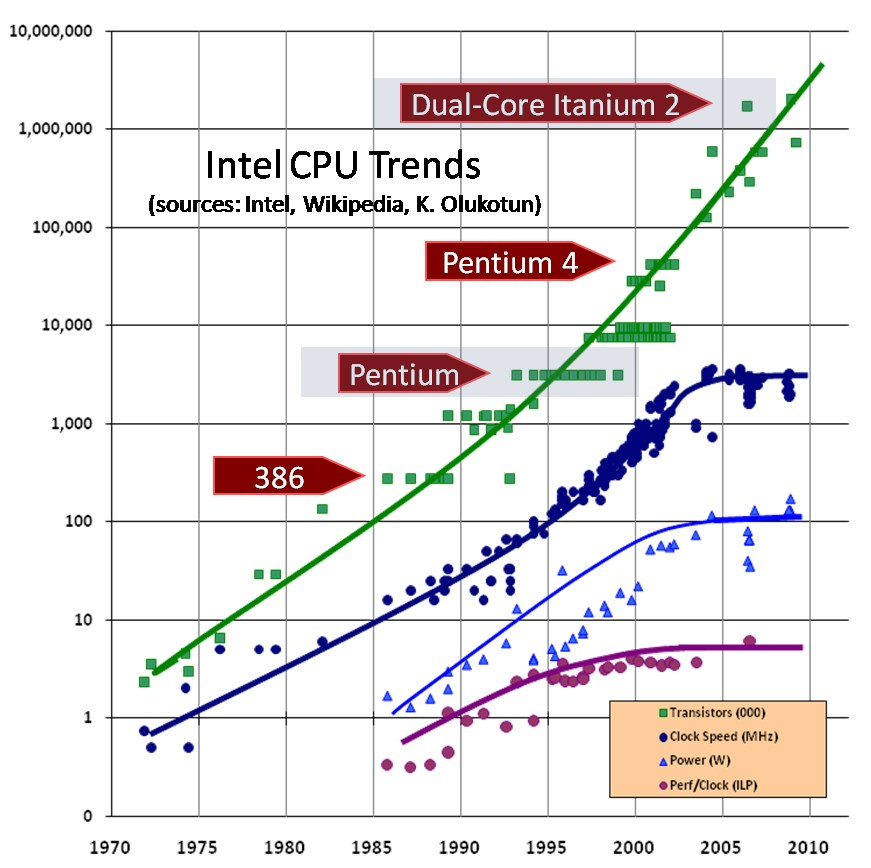
\includegraphics[width=0.75\linewidth]{imgs/CPU-Scaling.jpg}
  \caption{Comparison of the historic scaling behaviour of different CPU-performance metrics. Figure adapted from
  \cite{CPU-Scaling}.
  }
  \label{fig:MoorLaw}
\end{figure}
The less-well known Dennard scaling \cite{Dennard1974} is coming to an end. It predicts a constant power density in MOSFET transistors. Therefore, power consumption and switching delay should improve when scaling down a transistor.
However, from around 2006 the predicted improvements disagree with the observation\cite{Bohr2007}.
One reason is that in the same paper, Dennard already had predicted that the RC-delay of interconnects would not scale to size.
Eventually the time that it takes a signal to travel through an electrical interconnect from one part of the processor to another, depending on the RC-delay given by Resistance times Capacitance, begins to limit the speed of computation. Additionally, decreasing feature size eventually leads to quantum behaviour like tunnelling and interference. In modern chips, the dielectric layers are only several atoms thick. Tunnelling currents prevent chip manufacturers from reducing the voltage. The heating from this voltage limits further downsizing. As thermal conduction is proportional to the surface area, smaller circuits are more challenging to cool. The electric resistance of Silicon decreases with temperature once it surpasses $\sim 160^{\circ}C$. The decreasing resistance then leads to an increasing current, further heating the Silicon, driving it into a destructive positive feedback loop called thermal runaway. 
Nonetheless, numerous techniques were developed to improve processor performance further. Including various forms of pipelining and parallelism. However, the proposals of what technology might succeed Silicon chips, are just as numerous as the technologies to improve Silicon processors.
For example, InGaAs transistors, organic semiconductors and Graphene pose interesting properties as transistor materials \cite{luisier2011ultimate}.
Furthermore, the search for an entirely new computational paradigm has become prominent.
Light-based computation, neuromorphic computation and, most interestingly for this thesis, quantum computation are active fields of research.

\subsubsection{Quantum Computing}
As was already noticed by Richard Feynman \cite{Feynmana}: Quantum mechanics possess a complexity different from what classical computers are good at simulating. He therefore concluded that one could attempt to use quantum mechanics for new complex simulations. Consider $n$ non-interacting bosons in a 2-level system: the number of possible states scales as the number of unique combinations of $n$ particles in either state, thus $2^n$ complex numbers are required to represent any state in the Hilbert space but $2^n * 64$Bit quickly exceeds memory constraints of any classical computer. However, a quantum computer using two-level systems or qubits as storage would only require $n$ qubits. 

Complexity theory can show the strength of Quantum Computation more formally: Some problems like the Halting Problem \cite{Turing1937} fundamentally cannot be solved and other problems like the Traveling Salesman \cite{Biggs1986} can, in general, be solved but doing so may take longer than an average human life or even the age of the universe. Complexity-theory sorts all problems in classes. Two of the most important are \textbf{P} and \textbf{NP}. While for \textbf{P} the time to solve a problem scales polynomial with the problem size, \textbf{NP} scales exponentially. Compared to Dennard-scaling, the size of solvable \textbf{NP}-problems scales linearly in time at best. While the relation of \textbf{P} and \textbf{NP} remains a million-dollar question \cite{10.1145/1562164.1562186}, some problems are commonly considered to be in \textbf{NP} and not in \textbf{P}. Typically for these problems, a given answer is easy to verify but hard to find. Interestingly Quantum Computing was shown to have a different set of complexity classes \cite{Bernstein1997}.
Thus, Quantum Computing promises not only to solve current computations faster but also access to solve problems from \textbf{NP}   that had previously been considered beyond reach. Quantum Computing may even be capable of solving problems more complex than \textbf{NP} in polynomial time.
\begin{figure}[H]
\centering
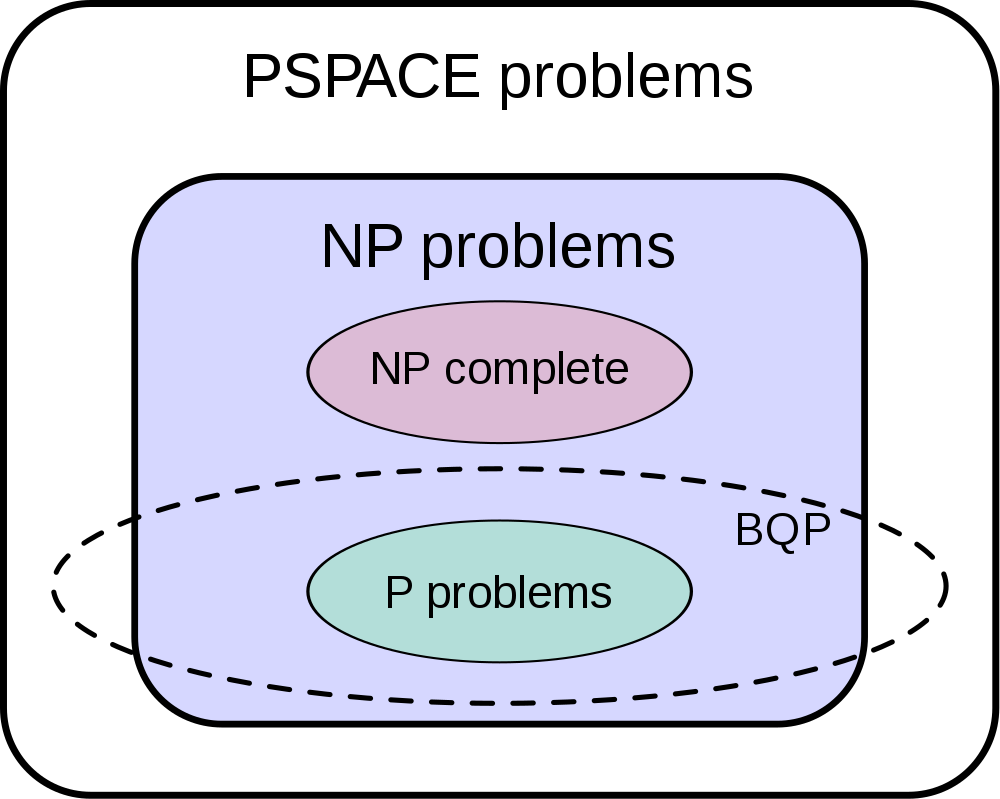
\includegraphics[width=0.6\linewidth]{imgs/BQP}
  \caption{Ven Diagram of classical and quantum complexity classes }
  \label{fig:BQP}
\end{figure}
Grover's \cite{Grover1997} and Shor's \cite{Shor1997} algorithm have shown that Quantum Computing can theoretically solve real-world problems faster than classical computation.
However, real-world quantum computers have so far been lacking. While in 2019, quantum supremacy was shown for the first time \cite{Martinis2019}, the applicability of this result remains debated.
So far, no quantum computer exists that could use Grover's or Shor's algorithm on significant real-world problems.
The problem is the noise in current quantum gates.
Many different implementations of qubits have been tried and tested,
but all of them are limited by noise and decoherence.
To counteract the noise, the field of quantum error-correcting codes has provided methods to perform accurate computation on noisy quantum gates \cite{shor1995scheme} with the caveat of requiring more qubits.
\subsubsection{Topological Quantum Computing}
While much research is conducted to reduce noise in current qubits, topological quantum computation is a comparatively new approach to reduce noise in the quantum gates. Non-local information storage and path independent exchange processes as operations provide resistance to external noise. Here thermal relaxation in the ground state is avoided by remaining in a degenerate ground state. The information is stored non locally in the phase between non-abelian quasi-particles and is thus protected from the environment. As the exchange phase depends on the permutations, it is independent of the exchange path and, thus, protected. The exchange of quasi-particles allows one to change the phase or perform Quantum Computation. 
\end{document}

